\documentclass{imports}
\usepackage[margin=1in]{geometry}

\title{\textbf{Analysis of Algorithms I}\\ k - Vertex Disjoin Path Problem}
\author{}
\date{}

\begin{document}
\maketitle
\allowdisplaybreaks % allow equations to be spit across files

    The given problem "The mutually avoiding path problem" or the "k - Vertex disjoint paths problem" is NP-Complete.
    We prove it by reducing 3-SAT to it. \cite{kddmain} \cite{stackoverflowkdd} \vspace{10pt}
    
    To prove the problem's NP-completeness, we need to first show that it is a search problem in NP. \vspace{10pt}
    
    \textbf{$k$ - Vertex disjoint paths problem in NP}\vspace{10pt}

    Given a solution of $k$ vertex disjoint paths, we simply check if each of the path's vertices and edges do exist in the main graph
    in polynomial time by traversing the adjacency matrix/list of the solution and comparing values with the adjacency matrix/list of the main graph.
    Also, to check the disjoint-ness, we can create an array of booleans of size $|V|$, where $|V|$ is as many vertices in the main graph. Each slot represents each vertex's presence
    in the $k$ disjoint paths. Now, we simply perform the travesal described above again and mark each vertex in the array. If during the traversal
    any one slot of the array already has a truth value present in it, then the paths are not disjoint. If until the end of the traversal that does not
    happen then they are a valid solution. Clearly, this is a polynomial time operation as well. As verifying the solution is a polynomial time
    operation the problem is in NP. \vspace{10pt}

    \textbf{The reduction} \vspace{10pt}

    Let the 3-SAT problem have $m$ clauses and $n$ variables. The overarching idea is to construct paths representing
    a satisfying assignment to each variable and to each clause and relating them in such a way that there should be $m+n$
    independent paths to represent a successful assignment. \vspace{10pt}

    \textbf{3-SAT problem input reduction in polynomial time}\vspace{10pt}
    
    For each variable $x_i$ ($1<=i<=n$) let there be a start and end vertex $vs_i, vt_i$. And let there be as many $vT_{ij}, vF_{ij}$
    ($1<=j<=m$) vertices as there are occurences of that variable in the $m$ clauses . We connect $vs_i$ to the first $vT_{ij}$ and connect
    that to the next $vT_{ij}$ and so on until the last $vT_{ij}$ and then connect that to $vt_i$. We repeat the same and connect the vertices $vs_i, vF_{ij}..., vt_i$. This way we have 2 paths going out from $vs_i$ and 2 paths converging on $vt_i$. Each of those paths represent a truth assignment
    or a false assignment for that variable. \vspace{10pt}

    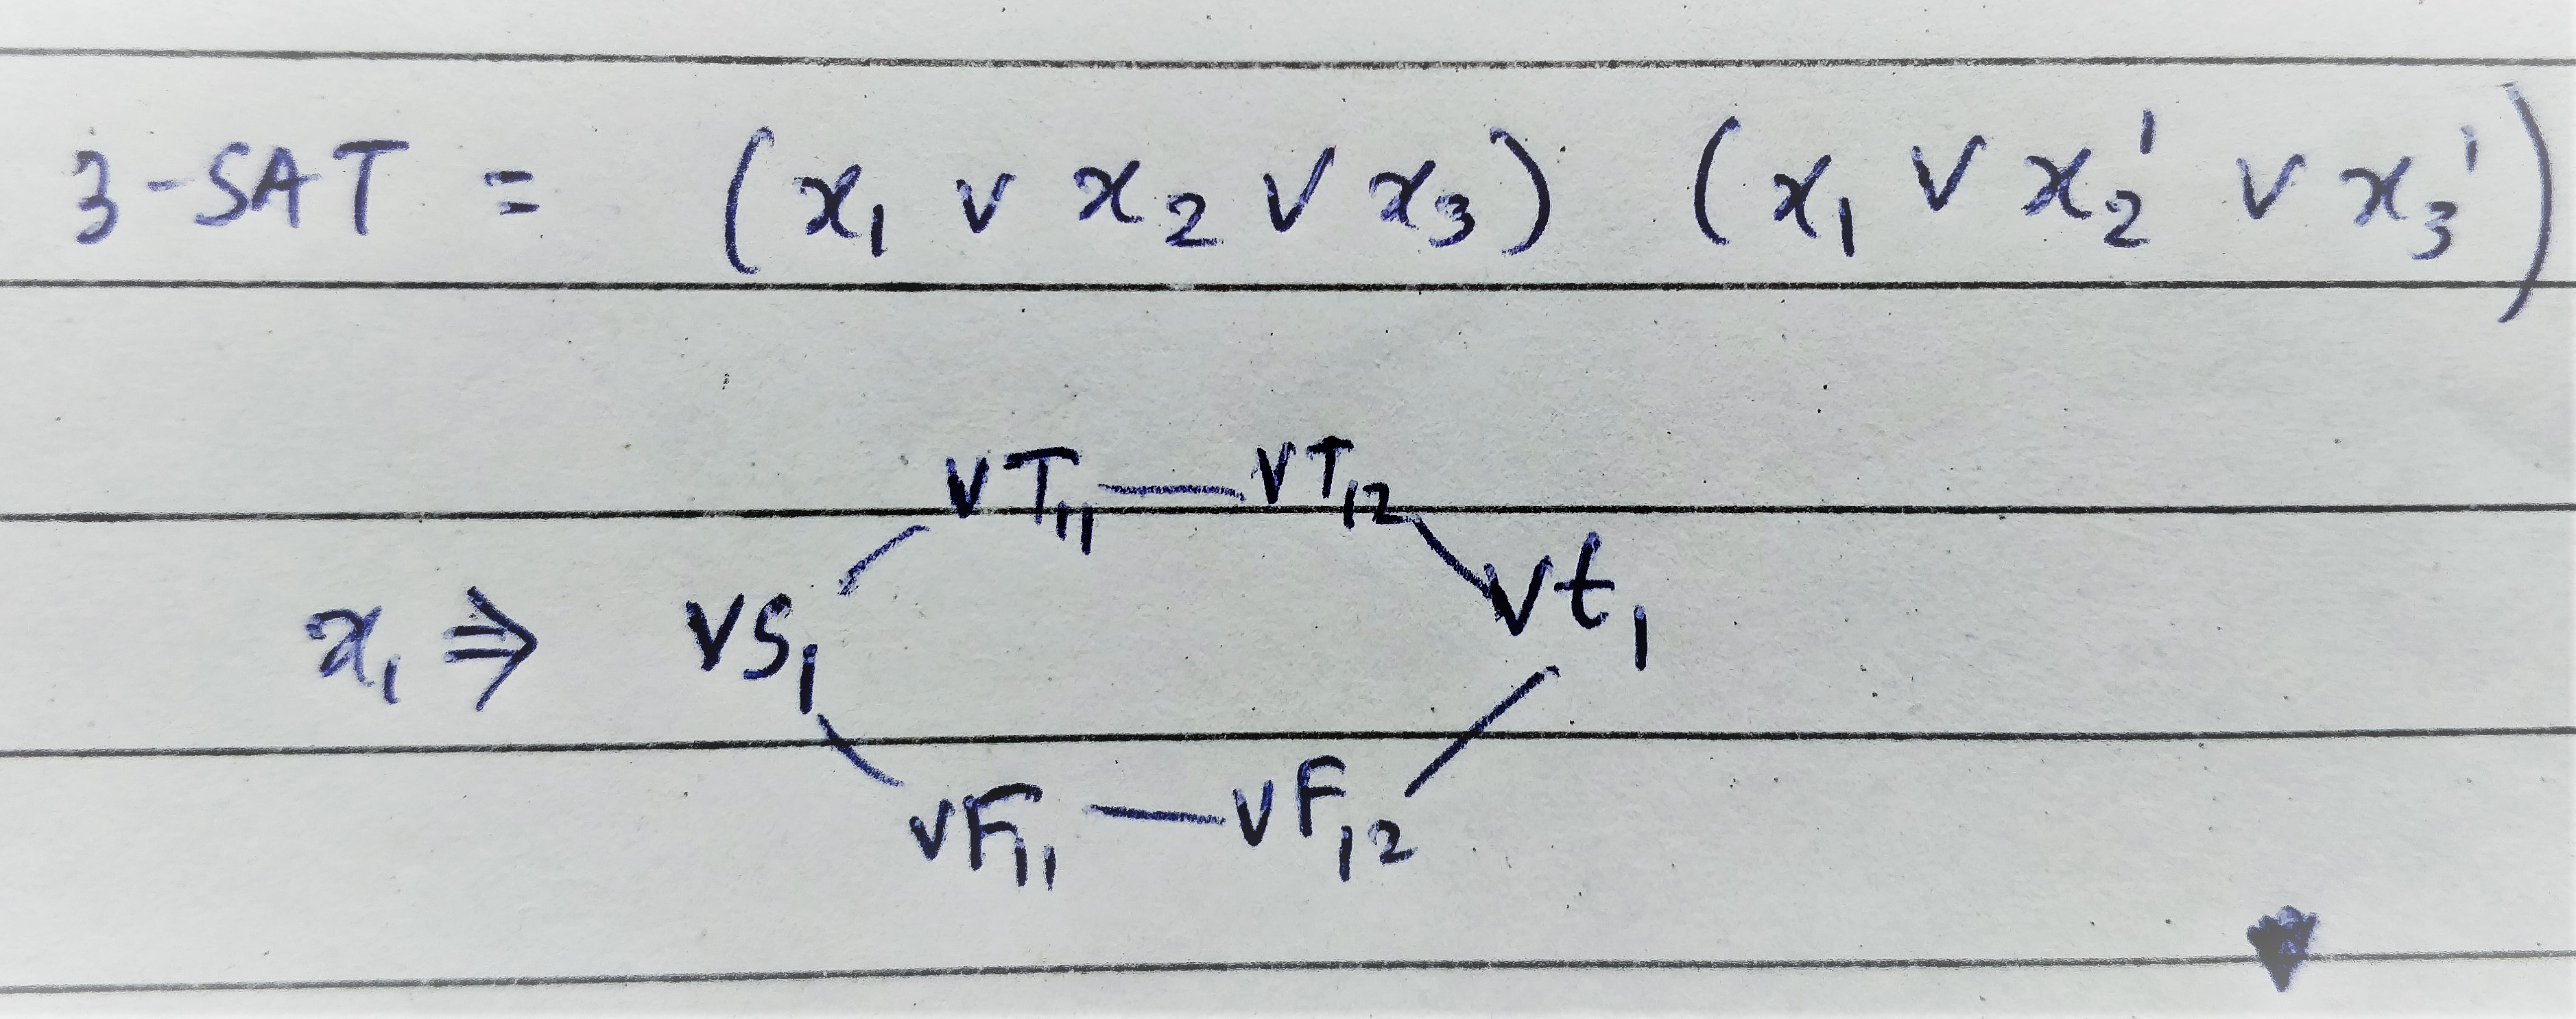
\includegraphics[width=\textwidth-25pt]{pic1.jpg} \vspace{10pt}

    Next, for each clause $c_i$ $(1<=i<=m)$ let there be a start and end vertex $cs_i, ct_i$. And let there be as many as $l_{ij}$ vertices as 
    there are literals in that clause ($j<=3$). We first connect $cs_i$ to all of the $l_{ij}$. Now if $l_{ij}$ is the unnegated variable
    $x_k$, then we connect it to $vF_{ki}$ (i.e the False vertex for variable $x_k$ for the current clause $i$). If $l_{ij}$ is the negated
    variable $x_k$, then we connect it to $vT_{ki}$ (i.e the Truth vertex for variable $x_K$ for the current clause $i$). Then we connect 
    the $vF_{ki}$ or the $vT_{ki}$ chosen to $ct_i$. We do this for all clauses and each literal variable for that clause.
    \vspace{10pt}.

    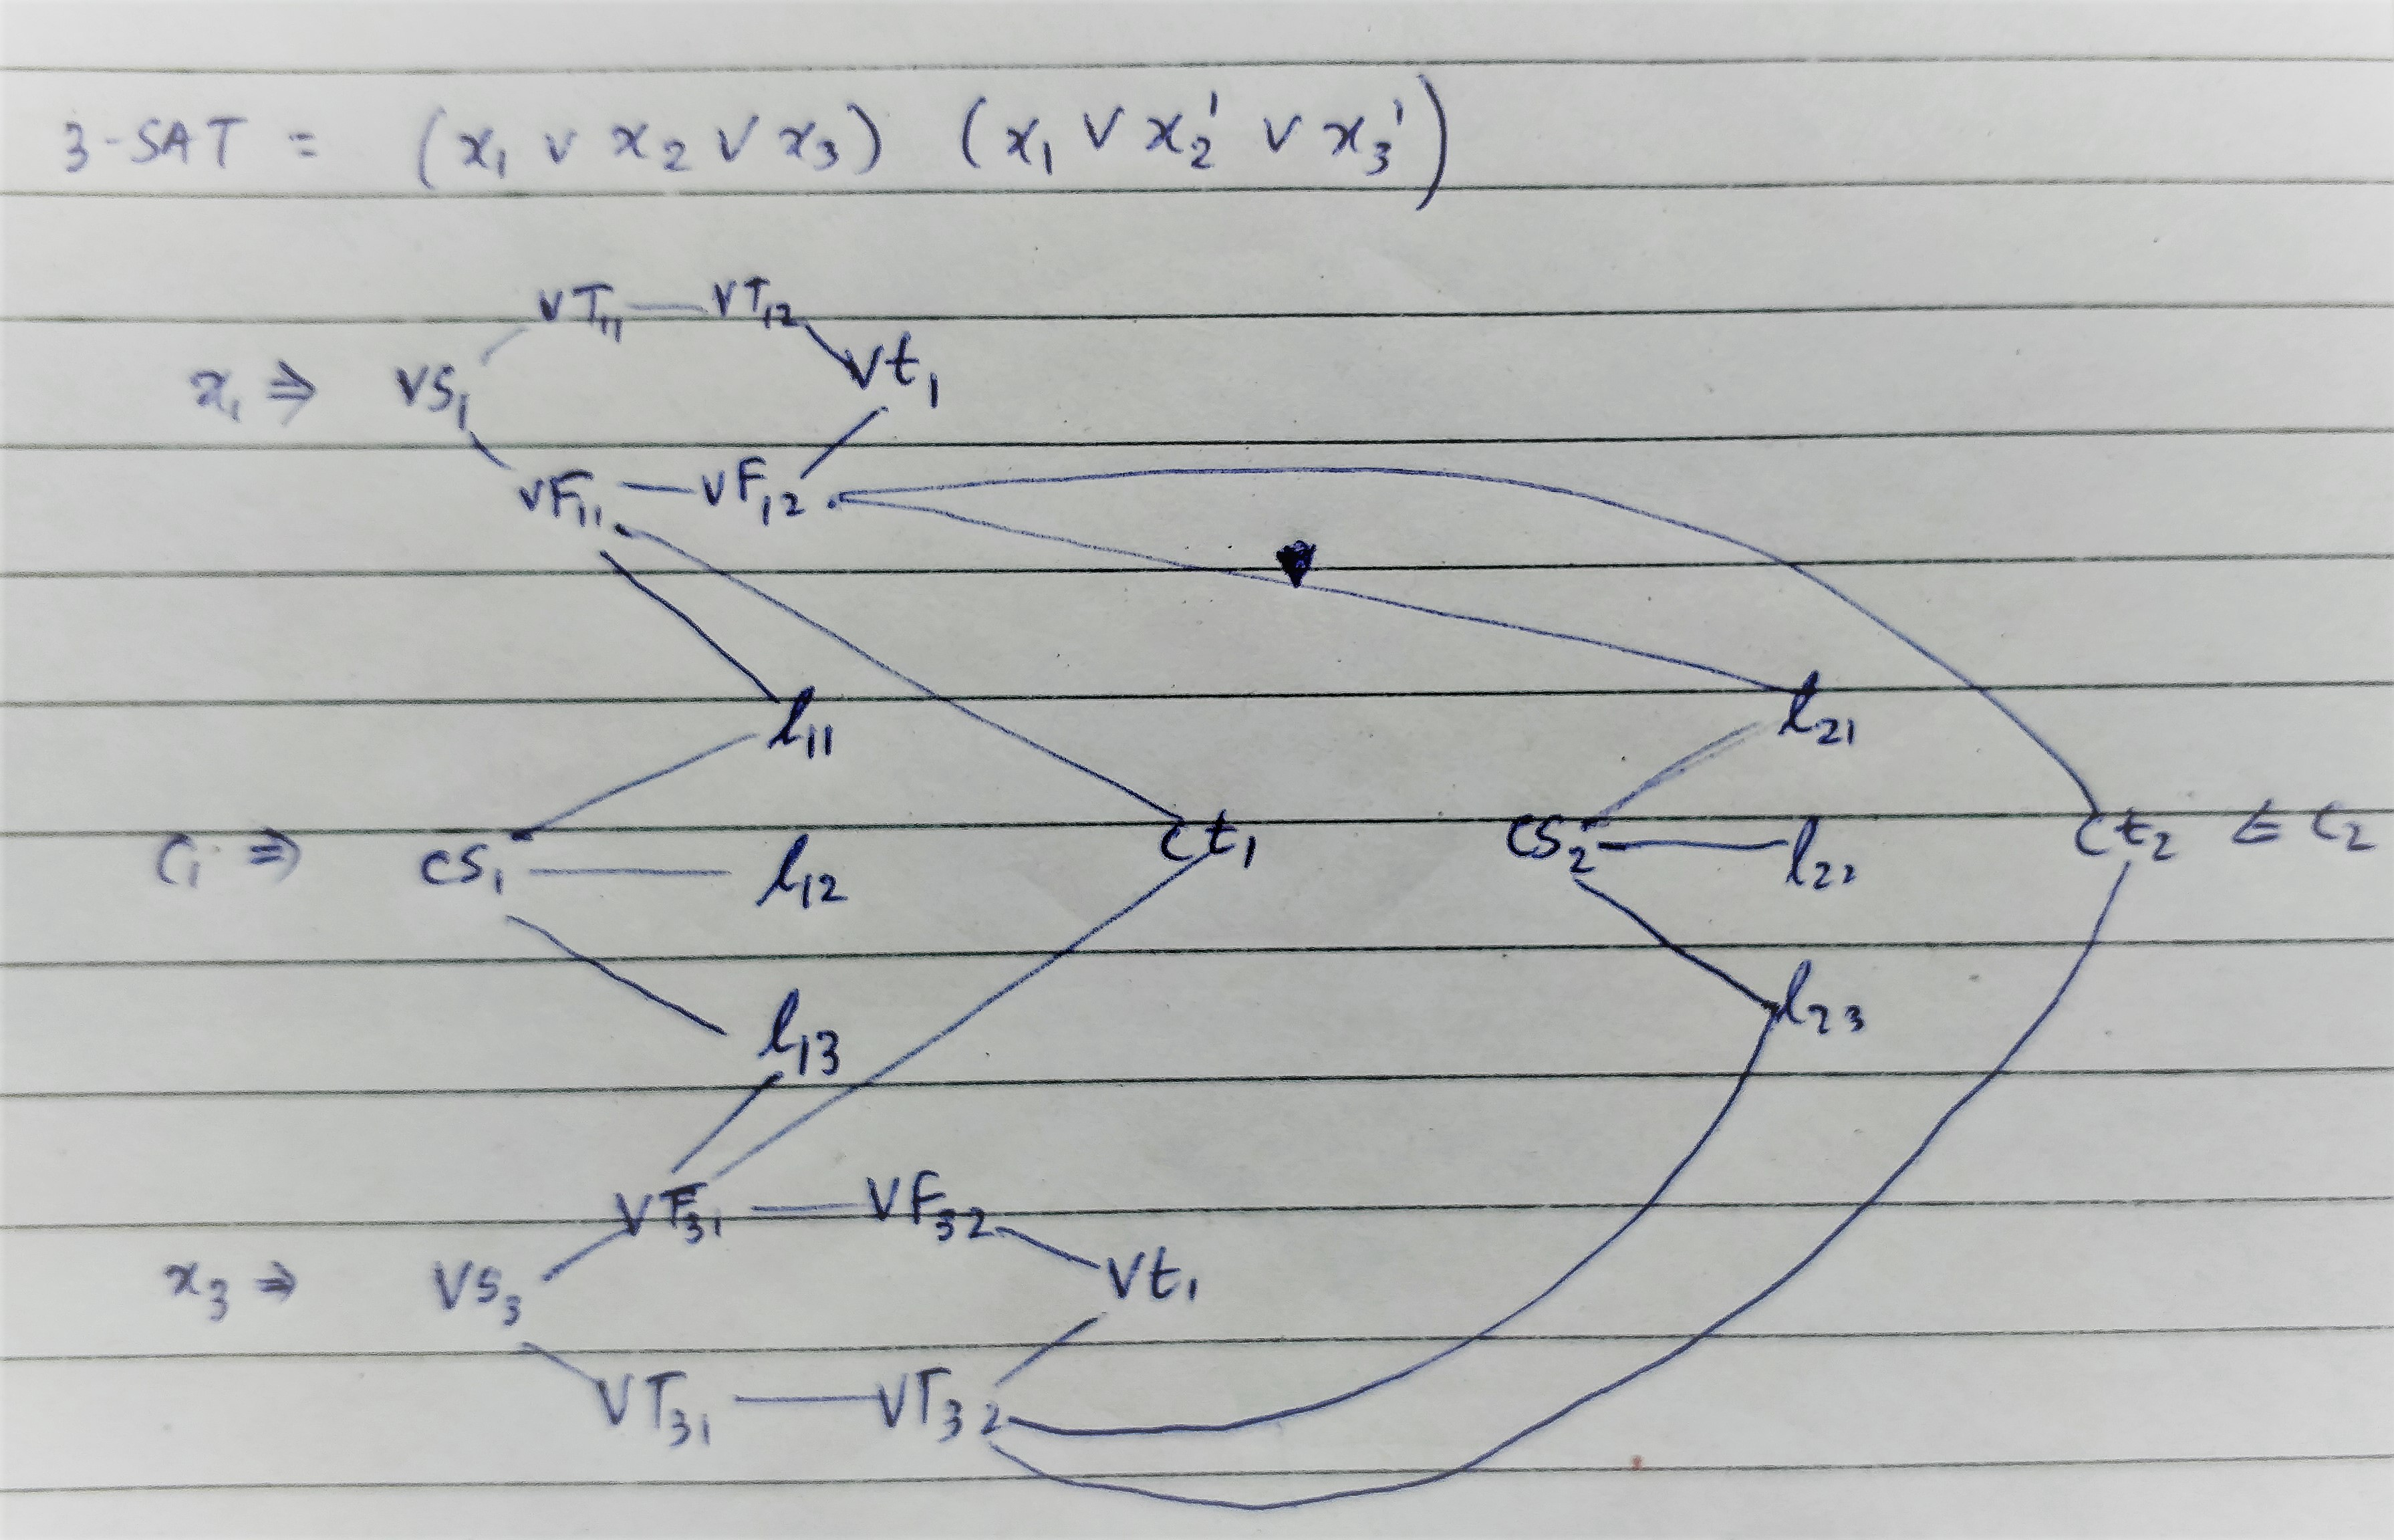
\includegraphics[width=\textwidth-25pt]{pic2.jpg} \vspace{10pt}

    This conversion of 3-SAT to the graph takes polynomial time as we add a fixed number of vertices for each clause and variable,
    i.e. polynomial in the size of the input. \vspace{10pt}

    \textbf{$k$ - Vertex disjoint paths problem solution reduction in polynomial time}\vspace{10pt}

    Now, given a $k = m+n$ vertex disjoint paths solution to the converted problem, extracting the truth assignment is polynomial time
    operation too. Visit each vertex $vs_i$ and check which way it branches out. If the path starting from the branch of $vT_{ij}$ is part of the solution, then variable $x_i$ has a truth value. If it branches out to $vF_{ij}$, then it has a false value. This is the 3-SAT satisfying assignment.
    \vspace{10pt}

    \textbf{Proof of solution} \vspace{10pt}

    Now, we need to prove that if there is a solution to the 3-SAT problem then there is a solution to the $k$ - Vertex disjoint paths problem as well and vice versa.\vspace{10pt}

    Let there be a truth assignment to the 3-SAT problem with $m$ clauses and $n$ variables. If in the problem, a variable $x_i$ has been assigned $True$, then in the reduced graph that we created it is equivalent to choosing the path $vs_i \to vT_{i1} \to  vT_{i2} \dots \to vt_i$ (All occurrences of $x_i$ have to be $True$). This means, that all the clauses that have this variable $x_i$ in the unnegated form still have the vertices left to choose from to create their own paths as they were connected to the corresponding $vF_{ij}$ vertex. Similarly, clauses which have this variable in the negated form and are thus connected to the $vT_{ij}$ can no longer form a  path as then have already been chosen. This is representative of the clause because if $x_i$ is True, then the clause with $x_i$ acheives its truth value from $x_i$ (and thus has a path using $vF_{ij}$). By using the truth assignment of the remaining variables in the same way, we see that we find $m+n=k$ paths that are vertex disjoint in the reduced graph. Thus the solution for a 3-SAT problem, provides the solution to the reduced $k$ - Vertex disjoint paths problem as well. \vspace{10pt}

    Let there be $k = m+n$ vertex-disjoint paths as a solution in the reduced graph generated. If from a source vertex in one of the paths, the branch with edge to $vT_{ij}$ is present, then that can be translated to setting the value of $x_i$ as $True$ in the 3-SAT problem. Checking any other path in the solution, it will either be for a different variable or a clause and as the path is disjoint, any assignment of a different variable will not interfere with our current variables assignment. As for the path starting from a corresponding clause vertex, it cannot include $vT_{ij}$ and thus includes $vF_{ij}$, which means that the literal is present in the unnegated state in the clause and thus is the right assignment to satisfy the clause. Similarly, we can get the corrseponding truth assignment for all variables based on the remaining disjoing paths in the graph and using the same logic, it will satisfy the 3-SAT formula. \vspace{10pt}
 
    This proves that the solution to $k$ - vertex disjoint paths problem exists iff a solution to the 3-SAT problem exits and proves that it is an NP-complete problem. \vspace{10pt}

    Therefore, the k - vertex disjoint paths problem is \textbf{NP-Complete}. \vspace{10pt}


    \textbf{Easier version of the problem - disjointed paths} \vspace{10pt}

    If the restriction of exact pairing is removed and we are allowed to pair any of the source vertices with any other target vertices,
    with vertex disjointedness maintained, it becomes a ploynomially solvable problem using max-flow min-cut. \vspace{10pt}

    We introduce a new parent source vertex $s_p$ which connects to all the $a_i$ start vertices, and a new parent target vertex $t$ 
    to which all the $b_i$ target vertices connect to. Then we split each vertex $v_i$ in the graph into $s_i, t_i$, where all incoming edges
    to that vertex connect to $s_i$, $s_i$ connects to $t_i$, and all the outgoing edges from that vertex go out from $t_i$.
    We also set the weights of all the edges to be 1. Finally we apply the Max-flow Min-cut algorithm. \vspace{10pt}
    
    Each augmenting path picked during the algorithm will ensure that the next augmenting path will not be able to use any of the edges and 
    vertices it has picked. This is because each edge only has a weight of 1. And each vertex was also split into $s_i, t_i$ with only one edge connecting
    them with a weight of 1. \vspace{10pt}
    
    For example, the augmenting path going from $s_p \to a_2 \to s_1 \to t_1 \to s_3 \to t_3 \to b_5 \to t_p$ resembles the path
    $a_2 \to v_1 \to v_3 \to b_5$ in the original graph. Vertices $v_1, v_3$ can't be used anymore in the next augmenting path because in the transformed
    graph the edge connecting their splits $s_1, t_1$ and $s_3, t_3$ is used up. This way the Max-flow Min-cut algorithm will only produce 
    vertex disjointed paths maxing out the flow $k$ from parent source $s_p$ to parent target $t_p$ giving us the $k$ vertex disjointed paths in polynomial time 
    (Max-flow Min-cut with fattest path heuristic with edge weights 1 is a polynomial time algorithm).\vspace{10pt}


    \textbf{Easier version of the problem - non-disjointed paths} \vspace{10pt}

    If there is no restriction on disjointness but the exact pairing provided has to be honored, even then the problem becomes a 
    polynomially solvable problem using something as simple as a DFS. In this case, we simply pick each start vertex, and apply DFS to find
    the end vertex per the pairing provided. We repeat this for each start node. DFS is a polynomial time algorithm and applying it $k$ times
    keeps it polynomial too.

    \vspace{10pt}
    \cite{team}
    \newpage
    \bibliographystyle{unsrt}
    \bibliography{npc}
\end{document}
